%
% Template for DAS course projects
%
\documentclass[a4paper,11pt,oneside]{book}
\usepackage[latin1]{inputenc}
\usepackage[english]{babel}
\usepackage{amsfonts}
\usepackage{amsmath}
\usepackage{amssymb,amsmath,color}
\usepackage{cite}
\usepackage{graphicx}
\graphicspath{{./figs/}}
\usepackage{float}
\usepackage{tikz}
\usepackage{listofitems} % for \readlist to create arrays
\usepackage[outline]{contour} %

\usepackage{xcolor}

\tikzstyle{node}=[thick,circle,draw=blue,minimum size=22,inner sep=0.5,outer sep=0.6]
\tikzstyle{pixel}=[thick,rectangle,draw=black,fill=white,minimum size=22,inner sep=0.5,outer sep=0.6]
\tikzstyle{node in}=[node,green!20!black,draw=green!30!black,fill=green!25]
\tikzstyle{node hidden}=[node,blue!20!black,draw=blue!30!black,fill=blue!20]
\tikzstyle{node out}=[node,red!20!black,draw=red!30!black,fill=red!20]
\tikzstyle{connect}=[thick,black] 
\tikzset{ % node styles
  node 1/.style={node in},
  node 2/.style={node hidden},
  node 3/.style={node out},
}
\def\nstyle{int(\lay<\Nnodlen?min(2,\lay):3)} % map layer number onto 1, 2, or 3



\begin{document}
\pagestyle{myheadings}

%%%%%%%%%%% Cover %%%%%%%%%%%
\thispagestyle{empty}                                                 
\begin{center}                                                            
    \vspace{5mm}
    {\LARGE UNIVERSIT\`A DI BOLOGNA} \\                       
      \vspace{5mm}
\end{center}
\begin{center}
  
\includegraphics[scale=.27]{logo_unibo}
\end{center}
\begin{center}
      \vspace{5mm}
      {\LARGE School of Engineering} \\
        \vspace{3mm}
      {\Large Master Degree in Automation Engineering} \\
      \vspace{20mm}
      {\LARGE Distributed Autonomous Systems} \\
      \vspace{5mm}{\Large\textbf{DISTRIBUTED CLASSIFICATION VIA NEURAL NETWORKS AND FORMATION CONTROL}}                  
      \vspace{15mm}
\end{center}
\begin{flushleft}                                                                              
     {\large Professors:}\\
     \textbf{\@ Giuseppe Notarstefano} \\
     \textbf{\@ Ivano Notarnicola} \\        
     \vspace{13mm}
\end{flushleft}
\begin{flushright}
      {\large Students:}\\
      {Simone Cenerini} \\
      {Giulia Cutini} \\
      {Riccardo Paolini} \\
\end{flushright}        %capoverso allineato a destra
\begin{center}
\vfill
      {\large Academic year \@2022/2023} \\
\end{center}



\newpage
\thispagestyle{empty}

%%%%%%%%%%% Abstract %%%%%%%%%%%%
\begin{center}
\chapter*{}
\thispagestyle{empty}
{\Huge \textbf{Abstract}}\\
\vspace{15mm}
\end{center}

\tableofcontents \thispagestyle{empty}
% \listoffigures\thispagestyle{empty}

%%%%%%%%%% Introduction %%%%%%%%%%
\chapter*{Introduction}
\addcontentsline{toc}{chapter}{Introduction}
\section*{Motivations} 

\section*{Contributions}



%%%%%%%%%% Chapter Title %%%%%%%%%%
\chapter{Distributed classification via Neural Network}

\begin{figure}
	\centering
	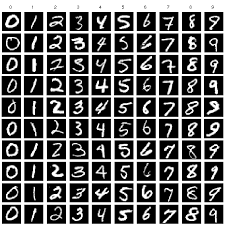
\includegraphics[scale=0.5]{mnist}
	\caption{Example of images from the \texttt{mnist} dataset}
	\label{mnist}
\end{figure}


In the first task we were asked to correctly classify a set of grayscale images. The dataset, downloaded from the Keras \texttt{mnist}, collects images of hand-written digits of $28\times28$ pixels each one, an example in figure \ref{mnist}. In order to perform our task we were asked to implement a distributed classification: given a predefined number of agents running each one a neural network with the same structure, we were asked to implement a Gradient Tracking algorithm to ensure consensus of the connection weights of the several neural networks runned separately by different agents.

\section{Initial setup}
The first step was to prepare the dataset by a reshape and a normalization of the images. We have flattened the $28\times28$ pixels grayscale images in order to obtain a $[784,1]$ column vector and we have normalized the pixels' intensities by dividing each intensity by $255$ in order to avoid a saturation of the activation function.

The classification we were asked to perform was a binary one: we have choose one among the ten digits (named as \texttt{target}) and assigned to it the label $1$, while, to all the other images, we have assigned the label $0$, in the following way:
\begin{equation}
y_i = 
\begin{cases}
1, & \text{if label = \texttt{target}} \\
0, & \text{otherwise}
\end{cases}
\end{equation}

As a consequence, we have performed a \textbf{balancing of the dataset}: in order to efficiently train our neural network we have equalized the representation of both the classes in the dataset ($50 \%$ of both since we have two classes). In order to do that we have undersampled the number of samples in the majority class. 

\section{Neural Network structure}

% NEURAL NETWORK SCHEME
\begin{figure}
\centering
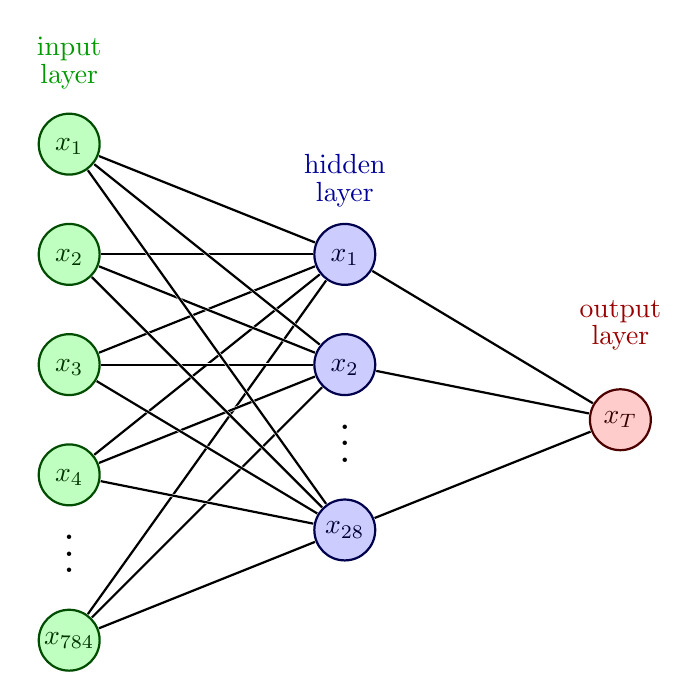
\begin{tikzpicture}[x=3.5cm,y=1.4cm]

\readlist\Nnod{5,3,1} % array of number of nodes per layer
\readlist\Nstr{n,m,k} 
\readlist\Cstr{\strut x,\strut x,{}} 
\def\yshift{0.5} % shift last node for dots


\foreachitem \N \in \Nnod{ 
\def\lay{\Ncnt} 
\pgfmathsetmacro\prev{int(\Ncnt-1)}
\message{\lay,}
\foreach \i [evaluate={\c=int(\i==\N); \y=\N/2-\i-\c*\yshift;
\index=(\i<\N?int(\i):"\Nstr[\lay]");
\x=\lay; \n=\nstyle;}] in {1,...,\N}{


% NODES
\ifnum\lay=1 % First Layer
  \ifnum\i=\N % Last neuron of first layer
    \node[node \n] (N\lay-\i) at (\x,\y) {$x_{784}$}; 
  \else
    \node[node \n] (N\lay-\i) at (\x,\y) {$\Cstr[\lay]_{\index}$};
  \fi
\fi

\ifnum\lay=2 % Second Layer
  \ifnum\i=\N % Last neuron of second layer
    \node[node \n] (N\lay-\i) at (\x,\y) {$x_{28}$}; 
  \else
    \node[node \n] (N\lay-\i) at (\x,\y) {$\Cstr[\lay]_{\index}$}; %empty
  \fi
\fi

\ifnum\lay=3 % Third Layer
  \node[node \n] (N\lay-\i) at (\x,\y) {$x_T$}; 
\fi
      % CONNECTIONS
      \ifnum\lay>1 % connect to previous layer
        \foreach \j in {1,...,\Nnod[\prev]}{ 
          \draw[connect,white,line width=1.2] (N\prev-\j) -- (N\lay-\i);
          \draw[connect] (N\prev-\j) -- (N\lay-\i);
        }
      \fi % nothing to connect first layer
      
    }
\ifnum\lay<\Nnodlen % draw dots for all layers except the last one
    \path (N\lay-\N) --++ (0,1+\yshift) node[midway,scale=1.5] {$\vdots$};
    \fi
}

%%PIXELS
%% Place pixels upstream of the first layer
%\foreach \i in {1,...,\Nnod[1]}{
%  \node[pixel] (P\i) at (0,\Nnod[1]/2-\i) {$p_\i$};
%  \draw[connect] (P\i) -- (N1-\i);
%}
%  
  % LABELS
% \pixel[above=5,align=center,black] at (N1-1.90) {flatten\\[-0.2em]image}
  \node[above=5,align=center,green!60!black] at (N1-1.90) {input\\[-0.2em]layer};
  \node[above=2,align=center,blue!60!black] at (N2-1.90) {hidden \\[-0.2em]layer};
  \node[above=10,align=center,red!60!black] at (N\Nnodlen-1.90) {output\\[-0.2em]layer};
  
\end{tikzpicture}
\caption{Scheme of the neural network for image classification}
\label{NN_scheme}
\end{figure}


The structure we have choose to develop for the neural network is a tapered one, represented in figure \ref{NN_scheme}. 
The first layer is composed by $784$ neurons, that is the dimension of the flattened image we give as input in the network. In this way each neurons of the first layer gets a single pixel as input. The second layer, the hidden one, has $28$ neurons since an higher number of neurons was useless in order to accomplish our task, while it increases a lot the computational effort required to train the network. The last layer has just one single neuron since we are asked to perform a binary classification, and so just a number between $0$ and $1$ is required as prediction.







\chapter{Formation Control}
ciao
  

%%%%%%%%%% Conclusions %%%%%%%%%%
\chapter*{Conclusions}
\addcontentsline{toc}{chapter}{Conclusions} 

%%%%%%%%%% Bibliography %%%%%%%%%%%
\bibliography{bibfile}{}
\bibliographystyle{plain}
\addcontentsline{toc}{chapter}{Bibliography}


%%%%%%%%%%%%%%%%%%%%%%%%%%%%%%%%%%%%%%

\end{document}